 \documentclass[11pt]{article} 
\usepackage[english]{babel}
\usepackage[utf8]{inputenc}
\usepackage[margin=0.5in]{geometry}
\usepackage{amsmath}
\usepackage{amsthm}
\usepackage{amsfonts}
\usepackage{amssymb}
\usepackage[usenames,dvipsnames]{xcolor}
\usepackage{graphicx}
\usepackage[siunitx]{circuitikz}
\usepackage{tikz}
\usetikzlibrary{calc,arrows.meta}
\usepackage[colorinlistoftodos, color=orange!50]{todonotes}
\usepackage{hyperref}
\usepackage[numbers, square]{natbib}
\usepackage{fancybox}
\usepackage{epsfig}
\usepackage{soul}
\usepackage[framemethod=tikz]{mdframed}
\usepackage[shortlabels]{enumitem}
\usepackage[version=4]{mhchem}
\usepackage{multicol}
\usepackage{mathtools}
\usepackage{comment}
\usepackage{enumitem}
\usepackage[utf8]{inputenc}
\usepackage{listings}
\usepackage{color}
\usepackage[numbers]{natbib}
\usepackage{subfiles}
\usepackage{tkz-berge}
\usepackage{algorithm}
\usepackage[noend]{algpseudocode}


\newtheorem{prop}{Proposition}[section]
\newtheorem{thm}{Theorem}[section]
\newtheorem{lemma}{Lemma}[section]
\newtheorem{cor}{Corollary}[prop]

\theoremstyle{definition}
\newtheorem{definition}{Definition}

\theoremstyle{definition}
\newtheorem{required}{Problem}

\theoremstyle{definition}
\newtheorem{ex}{Example}

\tikzset{
	vertex/.style={circle,draw,minimum size=16, inner sep=0pt,font=\normalsize},
	every node/.style={draw=none,rectangle,font=\scriptsize,outer sep=0pt,inner sep=2pt},
	directed/.style={arrows={-Stealth[length=7pt]},font=\small},
	caption/.style={text width=6cm,align=center,rectangle,draw}
}


\setlength{\marginparwidth}{3.4cm}
%#########################################################

%To use symbols for footnotes
\renewcommand*{\thefootnote}{\fnsymbol{footnote}}
%To change footnotes back to numbers uncomment the following line
%\renewcommand*{\thefootnote}{\arabic{footnote}}

% Enable this command to adjust line spacing for inline math equations.
% \everymath{\displaystyle}

% _______ _____ _______ _      ______ 
%|__   __|_   _|__   __| |    |  ____|
%   | |    | |    | |  | |    | |__   
%   | |    | |    | |  | |    |  __|  
%   | |   _| |_   | |  | |____| |____ 
%   |_|  |_____|  |_|  |______|______|
%%%%%%%%%%%%%%%%%%%%%%%%%%%%%%%%%%%%%%%

\title{
\normalfont \normalsize 
\textsc{CSCI 3104 Spring 2022 \\ 
Instructors: Profs. Chen and Layer} \\
[10pt] 
\rule{\linewidth}{0.5pt} \\[6pt] 
\huge Quiz 17 - Balanced versus Unbalanced Partitioning \\
\rule{\linewidth}{2pt}  \\[10pt]
}
%\author{Your Name}
\date{}

\begin{document}
\definecolor {processblue}{cmyk}{0.96,0,0,0}
\definecolor{processred}{rgb}{200, 0, 0}
\definecolor{processgreen}{rgb}{0, 255, 0}
\DeclareGraphicsExtensions{.png}
\DeclareGraphicsExtensions{.gif}
\DeclareGraphicsExtensions{.jpg}

\maketitle


%%%%%%%%%%%%%%%%%%%%%%%%%
%%%%%%%%%%%%%%%%%%%%%%%%%%
%%%%%%%%%%FILL IN YOUR NAME%%%%%%%
%%%%%%%%%%AND STUDENT ID%%%%%%%%
%%%%%%%%%%%%%%%%%%%%%%%%%%
\noindent
Due Date \dotfill March 18 \\
Name \dotfill \textbf{Chengming Li} \\
Student ID \dotfill \textbf{109251991} \\


\tableofcontents

\section{Instructions}
 \begin{itemize}
	\item The solutions \textbf{should be typed}, using proper mathematical notation. We cannot accept hand-written solutions. \href{http://ece.uprm.edu/~caceros/latex/introduction.pdf}{Here's a short intro to \LaTeX.}
	\item You should submit your work through the \textbf{class Canvas page} only. Please submit one PDF file, compiled using this \LaTeX \ template.
	\item You may not need a full page for your solutions; pagebreaks are there to help Gradescope automatically find where each problem is. Even if you do not attempt every problem, please submit this document with no fewer pages than the blank template (or Gradescope has issues with it).

	\item You \textbf{may not collaborate with other students}. \textbf{Copying from any source is an Honor Code violation. Furthermore, all submissions must be in your own words and reflect your understanding of the material.} If there is any confusion about this policy, it is your responsibility to clarify before the due date. 

	\item Posting to \textbf{any} service including, but not limited to Chegg, Discord, Reddit, StackExchange, etc., for help on an assignment is a violation of the Honor Code.

\end{itemize}

\newpage
\section{Standard 17 - Balanced versus Unbalanced Partitioning}
\begin{required}
Suppose that we modify the Merge-Sort algorithm so that the algorithm chooses a $(2, n-2)$ split for two levels of recursion and then a $(n/2,~n/2)$ split at the next level,  and this repeats so  a $(2, n-2)$ split is chosen for the next two levels, then a $(n/2,~n/2)$ split for one level, etc. \\

\noindent \textbf{Your job} is to write down a recurrence relation for this modified Merge-Sort algorithm and give its asymptotic solution, i.e., give your answer as $\Theta(f(n))$ for some function $f$. Show your work.\end{required}

\begin{proof}[Answer]
%Your answer here
\begin{center}
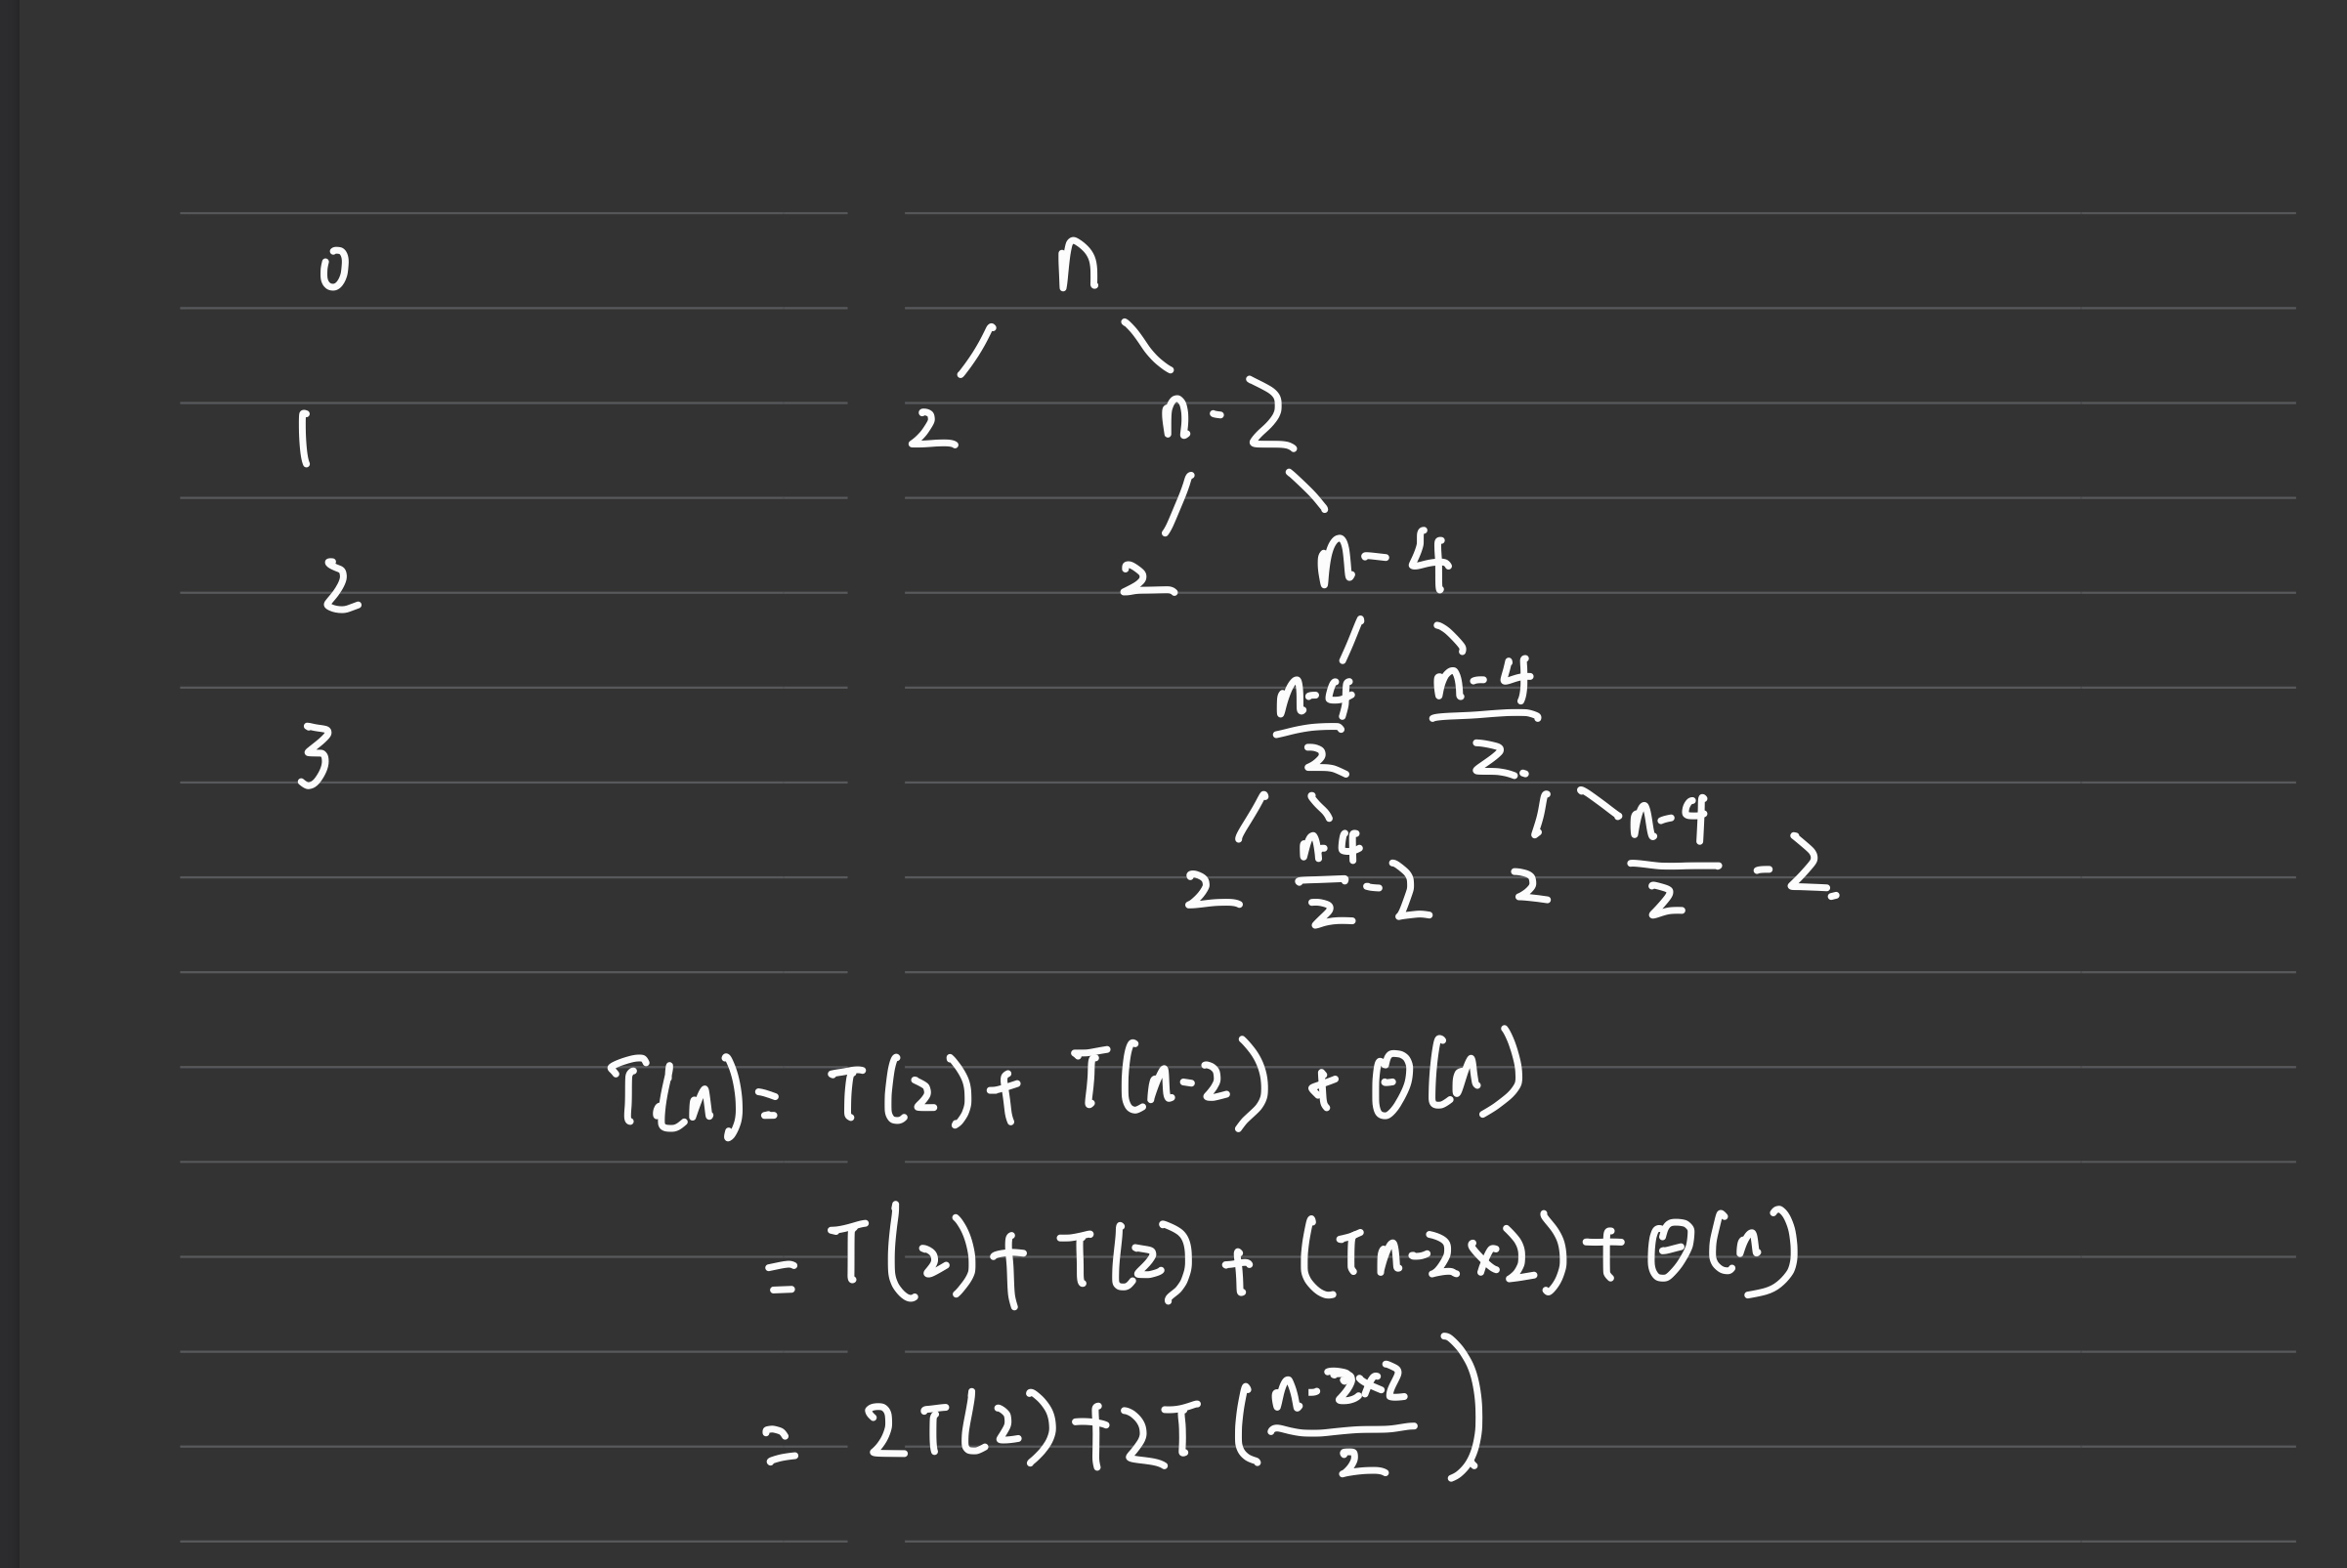
\includegraphics[width=0.7\textwidth]{IMG_0508.PNG}
\end{center}


\begin{align*}
T_{(2,n-2)}(n) = \begin{cases}
\Theta(n)& : n \leq 2.\\
T(2) + T(n-2) +\Theta(n)& : n > 2 
\end{cases}
\end{align*}

\begin{align*}
T_{(n/2,n/2)}(n) = \begin{cases}
\Theta(n)& : n \leq 2.\\
2T(\frac{n}{2}) + \Theta(n) & : n > 2 
\end{cases}
\end{align*}

\begin{align*}
T(n) &= T(2) + T(n-2) + \Theta(n)\\
&= 2T(2) + T(n-2*2) + \Theta(n)\\
&= 2T(2) + 2T(\frac{n-4}{2}) +2\Theta(n)
\end{align*}

\textbf{For finding the asymptotic solution, we could ignore the term T(2) and left with $2T(\frac{n-4}{2}).$}
\textbf{Finding the depth of tree first}
\begin{align*}
\frac{n-4}{2^{(1/3)k}} & \leq 2\\
n-4 &< 2^{(1/3)k+1}\\
log_2\left(n-4\right) &\leq ((1/3)k+1)\\
k &\geq 3 (log_2\left(n-4\right)-1)\\
k &\approx   3 (log_2\left(n-4\right)-1)
\end{align*}

\textbf{Total run time is:\\}
\begin{align*}
3 (log_2\left(n-4\right)-1) \cdot n
\end{align*}
approximate(n-4) to n and ignore -1\\
\begin{align*}
\lim _{n\to \infty }\left(\frac{3\:\left(log_2\left(n\right)\right)\cdot n\:}{nlog_2n}\right) &= 3
\end{align*}
\textbf{Asymptotic Solution is:\\}
\begin{align*}
3 (log_2\left(n-4\right)-1) \cdot n \in  \Theta(nlog_2(n))
\end{align*}
\end{proof}

%Include an Image: \includegraphics{ImageFileName}
%Include an Image and Rotate 90 degree: \includegraphics[angle=90]{ImageFileName}
%Include an Image, Rotate by 180 degrees, and scale by 50\% \includegraphics[scale=0.5, angle=90]{ImageFileName}



%%%%%%%%%%%%%%%%%%%%%%%%%%%%%%%%%%%%%%%%%%%%%%%%%%
\end{document} % NOTHING AFTER THIS LINE IS PART OF THE DOCUMENT



